%; whizzy chapter
% -initex iniptex -latex platex -format platex -bibtex jbibtex -fmt fmt
% 以上 whizzytex を使用する場合の設定。

%     Tokyo Debian Meeting resources
%     Copyright (C) 2011 Junichi Uekawa
%     Copyright (C) 2011 Nobuhiro Iwamatsu

%     This program is free software; you can redistribute it and/or modify
%     it under the terms of the GNU General Public License as published by
%     the Free Software Foundation; either version 2 of the License, or
%     (at your option) any later version.

%     This program is distributed in the hope that it will be useful,
%     but WITHOUT ANY WARRANTY; without even the implied warranty of
%     MERCHANTABILITY or FITNESS FOR A PARTICULAR PURPOSE.  See the
%     GNU General Public License for more details.

%     You should have received a copy of the GNU General Public License
%     along with this program; if not, write to the Free Software
%     Foundation, Inc., 51 Franklin St, Fifth Floor, Boston, MA  02110-1301 USA

%  preview (shell-command (concat "evince " (replace-regexp-in-string "tex$" "pdf"(buffer-file-name)) "&"))
% 画像ファイルを処理するためにはebbを利用してboundingboxを作成。
%(shell-command "cd image201109; ebb *.png")

%%ここからヘッダ開始。

\documentclass[mingoth,a4paper]{jsarticle}
\usepackage{monthlyreport}

% 日付を定義する、毎月変わります。
\newcommand{\debmtgyear}{2011}
\newcommand{\debmtgmonth}{12}
\newcommand{\debmtgdate}{17}
% (+ (* (- 2011 2005) 12) 12 -1) started from zero
\newcommand{\debmtgnumber}{83}

\begin{document}

\begin{titlepage}
\thispagestyle{empty}
% タイトルページ:編集必要な部分は最初のマクロに飛ばすこと

\vspace*{-2cm}
第\debmtgnumber{}回 東京エリア Debian 勉強会資料\\
\hspace*{-2cm}
\includegraphics[width=210mm]{image201003/debsen.eps}\\
\hfill{}\debmtgyear{}年\debmtgmonth{}月\debmtgdate{}日

% ここはアップデートすること
\rotatebox{10}{\fontsize{30}{30} {\gt 特集1: 2011年の振り返り}}

\rotatebox{10}{\fontsize{30}{30} {\gt 特集2: quiltでportingしてみた}}

\rotatebox{10}{\fontsize{30}{30} {\gt 特集3: 月刊Debhelper}}

\vspace*{-2cm}
\hfill{}
\includegraphics[height=6cm]{image200502/openlogo-nd.eps}
\end{titlepage}

\dancersection{Introduction}{上川 純一}

\begin{multicols}{2}
 

 今月のDebian勉強会へようこそ。これからDebianの世界にあしを踏み入れると
 いう方も、すでにどっぷりとつかっているという方も、月に一回Debianについ
 て語りませんか?

 Debian勉強会の目的は下記です。

 \begin{itemize}
 \item \underline{Debian Developer} (開発者)の育成。
 \item 日本語での「\underline{開発に関する情報}」を整理してまとめ、アップデートする。
 \item \underline{場}の提供。
 \begin{itemize}
  \item 普段ばらばらな場所にいる人々が face-to-face で出会える場を提供
	する。
  \item Debian のためになることを語る場を提供する。
  \item Debianについて語る場を提供する。
 \end{itemize}
 \end{itemize}		

 Debianの勉強会ということで究極的には参加者全員がDebian Packageをがりがり
 と作るスーパーハッカーになった姿を妄想しています。情報の共有・活用を通し
 て Debianの今後の能動的な展開への土台として、「場」としての空間を提供す
 るのが目的です。

\end{multicols}

\newpage

\begin{minipage}[b]{0.2\hsize}
 \definecolor{titleback}{gray}{0.9}
 \colorbox{titleback}{\rotatebox{90}{\fontsize{80}{80} {\gt デビアン勉強会} }}
\end{minipage}
\begin{minipage}[b]{0.8\hsize}
\hrule
\vspace{2mm}
\hrule
\begin{multicols}{2}
\tableofcontents
\end{multicols}
\vspace{2mm}
\hrule
\end{minipage}

\dancersection{事前課題}{野島 貴英}

今回の事前課題は以下です:
\begin{enumerate}
 \item 今年パッケージ化した、あるいは、使い込んだDebianパッケージを5つまであげて、そこで出会った課題について200文字以内に解説してください。
\end{enumerate}
この課題に対して提出いただいた内容は以下です。
\begin{multicols}{2}
{\small
\begin{prework}{Kazuo Ishii}
emacs $B>o$K%+%9%?%^%$%:$rB3$1$F$$$^$9!#$3$l$r$I$l$@$1;H$$$3$J$9$+$,!"2]Bj$G$9!#(B
\end{prework}
\begin{prework}{Aru}
\begin{itemize}
\item postfix$B$N%=!<%9%3!<%I$r$$$8$C$F%Q%C%1!<%82=$5$;$F%$%s%9%H!<%k$7$J$*$7$^$7$?!#(B
\item $B!{(BCN$B$N2s@~>e$G(BSMTP$B%5!<%P$r9=C[$9$k:]$O(BOP25B$B$N4X78>e(BOCN$B$N(BSMTP$B%5!<%P$rDL$5$J$1$l$P$J$i$J$$$N$G$9$,!"$=$N(BSMTP$B%5!<%P$,FC<l$J;EMM$N$h$&$G(Bpostfix$B$N@_Dj$rJQ$($k$@$1$G$O%5!<%P$KCF$+$l$F$7$^$$$^$9!#$=$3$G!"!{(BCN$B$N%5!<%P8~$1$K%=!<%9%3!<%I$r$$$8$j$^$7$?!#(B
\end{itemize}
\end{prework}

\begin{prework}{koedoyoshida}
\begin{itemize}
\item Unbound:\\
$B;E;v$GI>2AMQ(BDNS$B$r7z$F$k$N$K;H$C$?$j!"(Bdnstudy$BEy$GH/I=$N4m81$J(BLT$B%M%?$H$7$F;HMQ!#(BBIND$B$KHf$Y$FNI$/$G$-$F$k$N$GFC$K2]BjEy$O$J$7(B
\item zabbix:\\
$B4pK\(Bstable$B$r;H$C$F$$$k$3$H!"$+$DH/E8ES>e$N%=%U%H$G$"$k$3$H$+$iK-IY$J$O$^$j%]%$%s%H$,M-$C$?!#$,4pK\E*$K$0$0$C$F2r7h$7$?$j!"I=<(>e$NLdBj$J$N$GL5;k$7$?$j$7$F$^$9!#(B\\
\end{itemize}
\end{prework}

\begin{prework}{yamamoto}
\begin{itemize}
\item $B:#G/%Q%C%1!<%82=$7$?(BDebian$B%Q%C%1!<%8(B: $BL5$7(B \\
$B$&!<$`!"<+J,@lMQ$N%Q%C%A$r$"$F$?%+!<%M%k%Q%C%1!<%8$0$i$$$C$9$M!#(B
$B9W8%$O$G$-$F$J$$$J!#(B

\item $B:#G/;H$$9~$s$@(BDebian$B%Q%C%1!<%8(B: devscripts pbuilder \\
devscripts $B$G%]%A%]%A$H(B sbuild $BMQ$K%Q%C%1!<%8$r:n$j!"(Bpbuilder $B$G:F%S%k%I$7$F$^$7$?!#(B
$B:#G/$O(B FTBFS $B$rD>$7$F$b$i$&(B BTS $B$r$?$^$K$9$k$N$H!"<+J,@lMQ%j%]%8%H%j$r:G?7$K(B 
$BJ]$D$@$1$G!"$$$C$Q$$$$$C$Q$$$G$7$?!#(B

\item $BMhG/;H$$9~$`M=Dj$N(BDebian$B%Q%C%1!<%8(B: sbuild buildd \\
$B$5$F!"CF$,$G$-$?$7!"FM7b$8$c!<!#(B
\end{itemize}
\end{prework}
\begin{prework}{henrich}
$B:#G/$O$"$^$j%Q%C%1!<%8$r$$$8$/$C$F$J$$$G$9!D%Q%C%1!<%82=$7$?$b$N$H(B 
$B$$$($P(BIRC$B%/%i%$%"%s%H$N(Bloqui$B$H$+$0$i$$$G$7$g$&$+!#$=$l$b(Bupstream$B$NJ}$,!"$[$H(B 
$B$s$I?w7A:n$C$F$$$?$@$$$F$$$?$N$G:Y$+$$=j$rD>$7$?$@$1$G$7$?!#(B

DEP5$B$X$NBP1~$dB>$N(BDEP$B$X$NBP1~$J$I$,:#8e%Q%C%1!<%8%/%*%j%F%#$r5s$2$k>e$G2]Bj(B 
$B$G$7$g$&$+!J<g$KLLE]$/$5$$0UL#$G!K(B
\end{prework}
\begin{prework}{$B$^$($@$3$&$X$$(B}
 12/8$B;~E@$N>u67(B
\begin{itemize}
\item $B%Q%C%1!<%8%s%0:Q$_(B
\begin{itemize}
\item python-funcparserlib : $B%F%9%H$G%3%1$kLdBj(B
\item python-webcolors
\end{itemize}
\item $B%Q%C%1!<%8%s%0ESCf(B
\begin{itemize}
\item python-ordereddict$B!'(BPython2.6$B$N$_(B
\item python-blockdiag : Python 2.6$B$O(Bpython-ordereddict$B$r!"(B2.7$B$OAH$_9~$_$N(B 
ordereddict$B$r;H$&$h$&$K%Q%C%1!<%8%s%0$9$k$K$O(Bdebian/control$B$I$&=q$1$P$$$$$s(B 
$B$@!)(B
\item python-{sec,act,nw}diag$B$*$h$S(B 
python-sphinxcontrib.{block,seq,act,nw}diag : python-blockdiag$BBT$A(B
\item python-tomahawk : nodetests$B$G%3%1$kLdBj(B
\end{itemize}
\end{itemize}
\end{prework}


}
\end{multicols}

\dancersection{最近のDebian関連のミーティング報告}{野島 貴英}
\subsection{東京エリアDebian勉強会81回目報告}

10月の東京エリアDebian勉強会は、筑波大学にて開催されました。Debianをよく知らない学生の方々が
参加される可能性があったため、若い人向けにDebianについておさらいの意味で、
Debianとは何かについて岩松さんが発表しました。この発表をきっかけに若い方々でDebianに興味を
持っていただき、ますますDebian Developer候補が増えて欲しいと思います。

また、岡部さんにはDebian上でHaskellの開発について現状・問題点を説明していただきました。
関数型言語の代表的な言語の一つであるHaskellをDebianでやってみようという方が増えると
良いなぁと思っています。坂口さんには、Debian上でのLaTeX環境についての紹介と、学校の課題を
自動生成する事について発表していただきました。坂口さんは学生ということで、今の学生さんが
どのようにLaTeX環境と付き合っているのかについて非常に参考になりました。

最後に岩松さんから月刊Debhelperの企画と発表がありました。Debianのパッ
ケージを開発する際に強力なツールであるDebhelperのコマンドについて、毎月
2コマンド以上持ち回りで説明が行われる事になりました。きっとこれで、Debianパッケージ
開発者が益々増えると良いなぁと思います。

\subsection{東京エリアDebian勉強会82回目報告}

11月の東京エリアDebian勉強会はOSC Tokyo/Fallにてセッション形式で行いました。
場所は明星大学、第一日目の11/19(土)の11:00-11:45にて行っています。
Debian JP Projectの活動の宣伝と、最近のDebian事情について岩松さんより発表
していただきました。最近のDebian事情について、これほどまとまった内容はないんじゃないか
と思うほどの内容でした。

 また、OSC Tokyo/Fallでは11/19〜11/20の2日間ブースも出しています。
LiveDVDの配布も行いました。11/19はあいにくの雨にも関わらず多くの人が訪れたようです。
これでDebianユーザがもっともっと増える事を期待しています。

% (query-replace-regexp "<.*?>" "")
% (query-replace-regexp "^[	 ]\+" "")

\dancersection{Debian Trivia Quiz}{野島 貴英}

ところで、みなさん Debian 関連の話題においついていますか?Debian関連の話
題はメーリングリストをよんでいると追跡できます。ただよんでいるだけではは
りあいがないので、理解度のテストをします。特に一人だけでは意味がわからな
いところもあるかも知れません。みんなで一緒に読んでみましょう。

今回の出題範囲は\url{debian-devel-announce@lists.debian.org} や \url{debian-devel@lists.debian.org}に投稿された
内容とDebian Project Newsからです。
\begin{multicols}{2}
 %; whizzy-master ../debianmeetingresume201101.tex
% $B0J>e$N@_Dj$r$7$F$$$k$?$a!"$3$N%U%!%$%k$G(B M-x whizzytex $B$9$k$H!"(Bwhizzytex$B$,MxMQ$G$-$^$9!#(B
%
% $B$A$J$_$K!"%/%$%:$OJL%V%i%s%A$G:n@.$7!"$N$A$K%^!<%8$7$^$9!#5U$K%^!<%8$7(B
% $B$J$$$h$&$K$7$^$7$g$&!#(B
% (shell-command "git checkout quiz-prepare")

\santaku
{11$B7n=*$o$j:"$K%k!<%H%U%!%$%k%7%9%F%`$N9=B$$K$D$$$F5DO@$r8F$s$G$^$9!#FbMF$O!)(B}
{/user$B$r:n$k(B}
{/bin,/sbin,/lib$B$N<BBN$r(B/usr$B0J2<$K0\F0$7$F!"Be$o$j$K%7%s%\%j%C%/%j%s%/$K$9$k(B}
{/etc$B$N<BBN$r(B/usr$B0J2<$K0\F0$7$F!"Be$o$j$K%7%s%\%j%C%/%j%s%/$K$9$k(B}
{B}
{$BB><gMW%G%#%9%H%j%S%e!<%7%g%s$,:NMQ8!F$Cf(B...}

\santaku
{sun-java6$B$,(BDebian$B%Q%C%1!<%8$H$7$FG[I[$G$-$J$/$J$j$^$7$?!#Be$o$j$K(BDebian$B$G?d>)$5$l$k(BJava$B$O(B?}
{openjdk}
{gcj-jdk}
{coco-java}
{A}
{$B;DG0$@!d!{(Bracle}

\santaku
{11/19$B$KD9$i$/3hF0$rDd;_$7$F$$$?%Q%C%1!<%8%A!<%`$,I|3h@k8@$r$7$^$7$?!#$I$l$G$7$g$&!)(B}
{CORBA packaging team}
{Ham-radio packaging team}
{SDL packaging team}
{C}
{$B$3$l$+$i$b4hD%$C$FM_$7$$$G$9$M(B}

\santaku
{10/28$B!A(B30$B$G(BMiniDebconf2011$B$,3+$+$l$^$7$?!#$I$3$N9q$G$7$g$&!)(B}
{$B%K%+%i%0%"(B}
{$B%$%s%I(B}
{$B%U%i%s%9(B}
{B}
{$BMhG/$OF|K\$,$$$$$J$!(B}

\santaku
{Wheezy$B%U%j!<%:$N0Y$N(BBSP$B$,3F9q$G3+$+$l$^$7$?!#%I%$%D$H$I$3!)(B}
{$B%U%i%s%9(B}
{$B%K%+%i%0%"(B}
{$B%]!<%i%s%I(B}
{C}
{Wheezy$B$N%U%j!<%:$O(B2012/6$B$J$N$G!"3+H/:n6H$O$*Aa$a$K(B}


\end{multicols}

%-------------------------------------------------------------------------------
\dancersection{2011年の振り返り}{まえだこうへい}
%-------------------------------------------------------------------------------
\index{debianjp@Debian JP} 
\index{とうきょうえりあ@東京エリアDebian勉強会}
\index{2011ねん@2011年}

今月で7年目のDebian勉強会が終了しました。

\subsection{基本的な数値}

Debian 勉強会は毎回事前課題事後課題を設定しており、予習復習を必要だと謳っている勉強会です。
実際にどれくらいの人が出席しているのか、またその人たちがどれくらい事前課
題・事後課題を提出しているのか、確認してみましょう。
\fgref{fig:attendandprepostwork}です。
値は一年の移動平均です。

結果を見ると参加者数は下降傾向にあり、事前課題の提出率は昨年からは横ばい傾向です。
事前課題をちゃんとやる常連参加者に収斂されてきているのでしょうか?
一方、事後課題(ブログ)の率はさらに低下しています。昨年、「ブログはもう流行らないのでしょうか」との一言がありましたが、まさにその通りかもしれません。

\begin{figure}[ht]
\begin{center}
 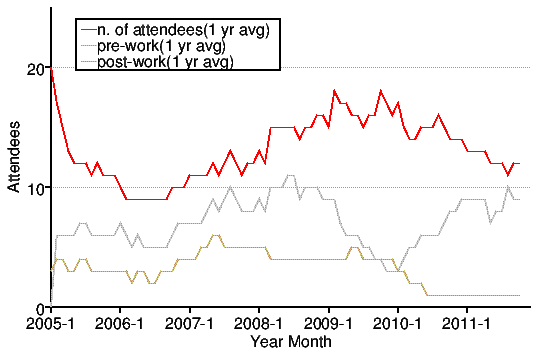
\includegraphics[width=0.7\hsize]{image201112/memberanalysis/attend.png}
\caption{東京エリアDebian勉強会事前課題・事後課題提出実績(12ヶ月移動平均)}\label{fig:attendandprepostwork}
\end{center}
\end{figure}

毎回の参加者の人数と、その際のトピックを見てみます。
今年も昨年同様、人数的には大きく増減はありませんが、10月の筑波大での開催での参加者が、昨年の筑波大でのつくらぐさんとの合同勉強会の時と同じ参加者数でした。新参の参加者を期待した筑波大生の参加は思ったほどではなかった一方、初参加なのにわざわざ都心から筑波大まで参加してくれた方が意外と多かった回でした。2009年から見ると、大学での開催はいつもより参加者数および初参加者が増えるので、来年以降も続けていくと良いでしょう。
また、リストをみると、毎月数名は初参加者も毎月いて、そのうち一部は2回目以降も参加する人がいることを考えると、先ほどの参加数が下降傾向にありつつ、事前課題の提出数が横ばいであるのは、ちゃんと事前課題を提出する人が常連になる傾向にあるのではないか、とも見れます。事前課題の提出率は維持しつつ、参加者数は増やしていく為の対策は必要でしょう。


会場を見ると、今年の会場は、あんさんぶる荻窪以外の公民館などの利用が増えました。
また、今年は3年前の草津温泉、昨年の木更津に続き、三回目のDebian温泉を伊東の山喜温泉で開催しました。
Debian Hack Cafeも6月ごろから月1回程度のペースで再開しているようです。

\begin{table}[ht]
\begin{minipage}{0.5\hsize}
 \caption{東京エリアDebian勉強会参加人数(2005-2006年)}\label{tab:count}
 \begin{center}
  \begin{tabular}{|l|c|p{10em}|}
 \hline
   & 参加人数 & 内容 \\
 \hline
   2005年1月 & 21 & 秘密\\
   2005年2月 & 10 & debhelper 1\\
   2005年3月 & 8 &  (早朝) debhelper 2、social contract\\
   2005年4月 & 6 & debhelper 3\\
   2005年5月 & 8 & DFSG、dpkg-cross、lintian/linda\\
   2005年6月 & 12 & alternatives、d-i\\
   2005年7月 & 12 & toolchain、dpatch\\
   2005年8月 & 7 & Debconf参加報告、ITPからアップロードまで\\
   2005年9月 & 14 & debconf\\
   2005年10月 & 9 & apt-listbugs、バグレポート、debconf翻訳、debbugs\\
   2005年11月 & 8 & DWN翻訳フロー、statoverride\\
   2005年12月 & 8 & 忘年会\\
   2006年1月 & 8 & policy、Debian勉強会でやりたいこと\\
   2006年2月 & 7 & policy、multimedia \\
   2006年3月 & 30 & OSC: debian勉強会、sid \\
   2006年4月 & 15 & policy、\LaTeX{} \\
   2006年5月 & 6 & mexico \\
   2006年6月 & 16 & debconf、cowdancer\\
   2006年7月 & 40 & OSC-Do: MacBook Debian \\
   2006年8月 & 17 & 13執念 \\
   2006年9月 & 12 & 翻訳、Debian-specific、oprofile \\
   2006年10月 & 23 & network、i18n会議、Flash、apt \\
   2006年11月 & 20 & 関西開催: bug、sid、packaging \\
   2006年12月 & 14 & 忘年会 \\
 \hline
  \end{tabular}
 \end{center}
\end{minipage}
\begin{minipage}{0.5\hsize}
 \caption{東京エリアDebian勉強会参加人数(2007-2008年)}\label{tab:count2007}
 \begin{center}
  \begin{tabular}{|l|c|p{10em}|}
 \hline
 & 参加人数 & 内容\\
 \hline
   2007年1月 & 15 & 一年を企画する \\
   2007年2月 & 13 & dbs, dpatch\\ 
   2007年3月 & 80 & OSC仮想化 \\
   2007年4月 & 19 & quilt, darcs, git\\
   2007年5月 & 23 & etch, pbuilder, superh \\   
   2007年6月 & 4 & エジンバラ開催:Debconf7 実況中継 \\
   2007年7月 & 18 & Debconf7 参加報告\\
   2007年8月 & 25 & cdn.debian.or.jp \\   
   2007年9月 & 14 & exim \\   
   2007年10月 & 30 & OSC Tokyo/Fall(CUPS) \\   
   2007年11月 & 19 & live-helper, tomoyo linux kernel patch, server\\
   2007年12月 & 11 & 忘年会\\
   2008年1月 & 23 & 一年を企画する \\
   2008年2/29,3/1 & 36 & OSC  \\
   2008年3月 & 37 & データだけのパッケージ、ライセンス \\
   2008年4月 & 17 & バイナリパッケージ \\
   2008年5月 & 20 & 複数のバイナリパッケージ \\
   2008年6月 & 10 & debhelper \\
   2008年7月 & 17 & Linux kernel patch / module パッケージ \\
   2008年8月 & 10 & Debconf IRC会議とDebian温泉 \\
   2008年9月 & 17 & po4a, 「Debian メンテナのお仕事」 \\
   2008年10月 & 11? & OSC Tokyo/Fall \\
   2008年11月 & 17 & 「その場で勉強会資料を作成しちゃえ」 Debian を使った \LaTeX{} 原稿作成合宿 \\
   2008年12月 & 12 & 忘年会 \\
 \hline
  \end{tabular}
 \end{center}
\end{minipage}
\end{table}

\begin{table}[t]
\begin{minipage}{0.5\hsize}
 \caption{東京エリアDebian勉強会参加人数(2009-2010年)}\label{tab:count2009}
 \begin{center}
  \begin{tabular}{|l|c|p{10em}|}
 \hline
 & 参加人数 & 内容\\
 \hline
   2009年1月 & 12 & 一年を企画する \\
   2009年2月 & 30 & OSC パッケージハンズオン\\ 
   2009年3月 & 23 & Common Lisp, パッケージ作成 \\
   2009年4月 & 15 & Java Policy, ocaml, 開発ワークフロー\\
   2009年5月 & 13 & MC-MPIパッケージ化、Erlang、Androidアプリ、DDTP \\   
   2009年6月 & 14 & DDTP・DDTSS、bsdstatsパッケージ、Debian kFreeBSD\\
   2009年7月 & 4 & スペインにてDebconf 9\\
   2009年8月 & 14 & スペイン Debconf 9 参加報告 \\   
   2009年9月 & 26 & GPGキーサインパーティー \\   
   2009年10月 & 30 & OSC Tokyo Fall\\
   2009年11月 & 12 & Octave, R, gnuplot, auto-builder \\
   2009年12月 & 10 & 忘年会\\
   2010年1月 & 17 &  東京大学にて新年会 \\
   2010年2月 & 11 & Debian温泉,ocaml,haskell \\
   2010年3月 & 12 & weka,fftw,dpkg v3 quilt \\
   2010年4月 & 15 & upstart,piuparts,debtags \\
   2010年5月 & 22 & 筑波大学,kernel \\
   2010年6月 & 12 & OSC-Doリハーサル  \\
   2010年7月 & 0 & キャンセル  \\
   2010年8月 & 3 & Debconf (NYC) \\
   2010年9月 & 30 & OSC Tokyo/Fall \\
   2010年10月 & 13 & 俺のDebianな一日 \\
   2010年11月 & 15 & ext4,btrfs,nilfs,ceph \\
   2010年12月 & 14 &  cacert, libsane \\
 \hline
  \end{tabular}
 \end{center}
\end{minipage}
\begin{minipage}{0.5\hsize}
 \caption{東京エリアDebian勉強会参加人数(2011年)}\label{tab:count2011}
 \begin{center}
  \begin{tabular}{|l|c|p{10em}|}
 \hline
 & 参加人数 & 内容\\
 \hline
   2011年1月 & 12 & 荻窪,Kinect,アンケートシステム,CACertサイン会 \\
   2011年2月 & 13 & 北新宿生涯学習館,HDFS,Debian Game Team \\
   2011年3月 & ? & OSC Tokyo/Spring,CACert ATE Tokyo \\
   2011年4月 & 12 & IIJ,backports,initramfs,月刊PPC64 \\
   2011年5月 & 15 & 戸山生涯学習館,Apache2モジュール,Debian on ニフクラ,Debian/m68k,月刊PPC64 \\
   2011年6月 & 17 & 東京オリンピックセンター,ドキュメント処理系,2011再計画 \\
   2011年7月 & 3 & DebConf11 \\
   2011年8月 & 12 & 荻窪,パッケージング関連, Debconf11報告 \\
   2011年9月 & 9 & 山喜旅館,Debian温泉2011 \\
   2011年10月 & 22 & 筑波大学,Haskell,LaTeX,レポート自動生成,月刊Debhelper開始 \\
   2011年11月 & ? & OSC Tokyo/Fall \\
   2011年12月 & 9 & スクウェア・エニックス,quiltでporting,月刊Debhelper,振り返り \\
 \hline
  \end{tabular}
 \end{center}
\end{minipage}
\end{table}


%-------------------------------------------------------------------------------
\dancersection{quiltでportingしてみた}{杉本典充}
%-------------------------------------------------------------------------------
\index{きるとでぽーてぃんぐしてみた@quiltでportingしてみた}
\index{ぽーてぃんぐ@porting}
\index{けーふりーびーえすでぃー@kfreebsd}
 
\subsection{はじめに}
本稿はdebianのパッケージ作成で使用しているパッチ管理ツールquiltの紹介、
およびquiltを用いてkfreebsdのportingパッチを作成しましたので発表します。

\subsection{Debianパッケージのフォーマット}

現在Debianで使用している主なソースパッケージフォーマットは2つです。
\footnote{東京エリアDebian勉強会 2010年03月号「dpkg ソース形式 ``3.0(quilt)''」 吉野与志仁}
\footnote{\url{http://wiki.debian.org/Projects/DebSrc3.0}}

\begin{itemize}
 \item{3.0(native):tarball1つで構成されたソースパッケージフォーマット}
  \begin{itemize}
   \item{packagename-version.tar.ext}
   \item{packagename-version.dsc}
  \end{itemize}
  \item{3.0(quilt):あるアップストリームのtarballとDebianパッケージ作成に
必要なtarballに分割しているソースパッケージフォーマット}
  \begin{itemize}
   \item{packagename-upstreamversion.orig.tar.ext}
   \item{packagename-upstreamversion.orig-component.tar.ext(任意)}
   \item{packagename-debianversion.debian.tar.ext}
   \item{packagename-debianversion.dsc}
  \end{itemize}
\end{itemize}

ソースパッケージフォーマットの詳細は `dpkg-source(1)' コマンドで確認することができます。
\footnote{manの記述には3.0(custom)、3.0(git)、3.0(bzr)というパッケージ形式の定義があるようです。}

アップストリームのソースコードを無修正のままDebianパッケージを作成した場合、
lintian処理でエラーになったり、Debianの開発ポリシーを満たせない場合が
あります(アップストリームのソースコードはIPv6で動作しない、など)。
そのときは、3.0(quilt)のソースパッケージフォーマットでパッケージを作成し、
必要なパッチを当ててからソフトウェアのビルド処理を行うことで対応させます。

\subsection{quiltパッケージ}
quiltはdebianパッケージを作成するときにパッチファイルを管理するツールとして
採用しているソフトウェアです。
Debianパッケージとして提供しており、aptでインストールできます。

\begin{commandline}
# apt-get update
# apt-get install quilt
\end{commandline}

quiltコマンドは複数のpatchファイルをスタックに積んだようなイメージで、
パッチの適用順番を管理します。
\footnote{東京エリアDebian勉強会 2007年01月号「パッチ管理ツールquiltの使い方」小林儀匡}

quiltコマンドを使うことで、パッケージ作成に必要なパッチが複数ある場合も
正しく適用でき、不要なパッチが出てきたときにそのパッチを取り除くことが容易に
なります。


\subsection{quiltの使用例:Debian GNU/kFreeBSD向けのportingパッチ作成}

\subsubsection{Debian GNU/kFreeBSDとは}
Debian Projectで開発しているOSはLinuxカーネルを用いた「Debian GNU/Linux」が有名ですが、
Linuxカーネル以外を用いたDebianがあります。その1つとしてFreeBSDカーネルを用いた「Debian GNU/kFreeBSD」
\footnote{\url{http://wiki.debian.org/Debian\_GNU/kFreeBSD}}があり、ユーザランドはDebianなので APT が使え、
デバイスやシステムコールといったカーネル特有の機能はFreeBSDカーネルに準じる、という特徴があります。
Debuan GNU/kFreeBSDは安定版のリリースには至っていませんが、日々開発が続けられています。

本稿では以降「Debian GNU/kFreeBSD」を「kfreebsd」と略記します。

\subsubsection{kfreebsdのporting作法}
Debianのporting関連情報およびkfreebsdのporting情報は以下にあります。

\begin{itemize}
 \item{\url{http://www.debian.org/ports/}}
 \item{\url{http://www.debian.org/ports/kfreebsd-gnu/}}
 \item{\url{http://glibc-bsd.alioth.debian.org/porting/}}
\end{itemize}

「\url{http://glibc-bsd.alioth.debian.org/porting/PORTING}」を読むと
kfreebsd向けにportingするには以下の確認および修正が行うようにとあります。

\begin{itemize}
 \item{Add our system name to checks here and there}
  \begin{itemize}
   \item{Makefileやスクリプト中のunameなどをチェックしてください。 }
  \end{itemize}
 \item{debian/control files}
  \begin{itemize}
   \item{debian/controlファイルでArchitectureをlinux専用ソフトウェアの場合は「linux-any」等、
CPUの違いのみでLinux、kfreebsdは関係なく使用できるソフトウェアの場合は「any-i386」等に変更してください。}
  \end{itemize}
 \item{Libraries, your beloved enemy}
  \begin{itemize}
   \item{libtool、aclocal.m4周りに対応してください。}
  \end{itemize}
 \item{Preprocessor Variables}
  \begin{itemize}
   \item{kfreebsdのシステムマクロは「\_\_FreeBSD\_kernel\_\_」、
バージョンマクロは「\_\_FreeBSD\_kernel\_version」なので対応してください。}
  \end{itemize}
 \item{Writing to devfs (kFreeBSD)}
  \begin{itemize}
   \item{FreeBSDカーネルでは(udevではなく)devfsを使うようにしてください。}
  \end{itemize}
 \item{RT signals}
  \begin{itemize}
   \item{FreeBSDカーネルは「POSIX RT (realtime) signals」がないので変更してください。}
  \end{itemize}
 \item{Get libc soname (6 or 6.1 on linux-gnu, 0.1 on kfreebsd-gnu, etc)}
  \begin{itemize}
   \item{使用するlibcの名前をハードコードしているプログラムがあれば修正してください。}
  \end{itemize}
\end{itemize}


\subsubsection{kfreebsdに対応させたいパッケージとその原因}

今回portingするパッケージは既にkfreebsd用パッケージとして存在している
icewmとなります。
icewmはウィンドウマネージャのソフトウェアで軽快な動作をするのが特徴です。

icewmではタスクバーにバッテリー残量アイコンを表示する機能がありますが
kfreebsdでは表示されません。linux-i386及びlinux-amd64では表示されるため
kfreebsdのポーティングが不完全の可能性があります。

まずはビルド準備とソースコードのダウンロードを行います。

\begin{commandline}
# apt-get update
# apt-get build-dep icewm
$ apt-get source icewm
\end{commandline}

ソースコードを「\_\_FreeBSD\_\_」及び「\_\_linux\_\_」grepすると、電源周りの処理で以下のマクロが検出されます。
\begin{commandline}
$ cd icewm-1.3.7/src
$ grep -nr __FreeBSD__ *
aapm.cc:30:#ifdef __FreeBSD__
aapm.cc:74:#if defined(__FreeBSD__) && defined(i386)
aapm.cc:99:#if defined(__FreeBSD__) && defined(i386)
aapm.cc:273:#ifndef __FreeBSD__
aapm.cc:333:#ifndef __FreeBSD__
aapm.cc:418:#ifndef __FreeBSD__
aapm.cc:463:#ifdef __FreeBSD__
aapm.cc:885:#ifndef __FreeBSD__
aapm.h:2:#if defined(linux) || (defined (__FreeBSD__)) || (defined(__NetBSD__) && defined(i386))
aapm.h:7:#if defined(__FreeBSD__) || defined(__NetBSD__) || defined(__OpenBSD_
(以下略)

$ grep -nr __linux__ *
(なにもなし)
\end{commandline}

\_\_FreeBSD\_\_マクロはFreeBSD OSを示すマクロですが、kfreebsdでは「\_\_FreeBSD\_kernel\_\_」がシステム(厳密にはカーネル)を示すマクロです。そのためマクロでシステムを切り分けているはずがkfreebsd向けのパッケージビルド時にLinuxカーネル向けの処理が有効なコードとしてビルドされてしまいバッテリー残量アイコンの表示がうまく動作していないようです。

そのため、今回はこのマクロを「PORTING」の記述に従って以下のような修正を行います。

\begin{commandline}
(修正前)#ifdef __FreeBSD__

(修正後)#if defined(__FreeBSD__) || defined(__FreeBSD_kernel__)
\end{commandline}
これで修正方針が定まりましたので、debianパッケージ作成に向けてパッチを作成していきます。

\subsection{quiltの登場}
今回は新規のパッチファイルとなるため、quiltのパッチスタックに新規追加します。

\begin{commandline}
$ cat debian/patches/series
#cvs_fixes
package_build_fixes
#misc_fixes
debian_defaults
#compiler_defaults
#iconify_on_wm_hint
#move-to-screen
i18n_updates
tray_hotfixes
imap_unseen
ifstate_exact_check
debian-changes-1.3.7~pre2-1.1

$ quilt new kfreebsd_porting_aapm
Patch kfreebsd_porting_aapm is now on top

$ cat debian/patches/series
#cvs_fixes
package_build_fixes
#misc_fixes
debian_defaults
#compiler_defaults
#iconify_on_wm_hint
#move-to-screen
i18n_updates
tray_hotfixes
imap_unseen
ifstate_exact_check
debian-changes-1.3.7~pre2-1.1
kfreebsd_porting_aapm
\end{commandline}
%$

これでパッチを新規に追加できました。

次にportingするために修正を行うソースファイルをquiltで管理するように登録処理をします。
その後「quilt edit ソースファイル」を実行すると、環境変数EDITORで登録したエディタが自
動で起動しますのでソースファイルの修正作業を行います。


\begin{commandline}
$ quilt add src/aapm.h
File src/aapm.h added to patch kfreebsd_porting_aapm

$ quilt edit src/aapm.h
File src/aapm.h is already in patch kfreebsd_porting_aapm

$ quilt refresh
Refreshed patch kfreebsd_porting_aapm

$ quilt add src/aapm.cc
File src/aapm.cc added to patch kfreebsd_porting_aapm

$ quilt edit src/aapm.cc
File src/aapm.cc is already in patch kfreebsd_porting_aapm

$ quilt refresh
Refreshed patch kfreebsd_porting_aapm
\end{commandline}

できたパッチファイル「kfreebsd\_porting\_aapm」を確認します。

\begin{commandline}
$ cat debian/patches/kfreebsd_porting_aapm
Index: icewm-1.3.7/src/aapm.h
===================================================================
--- icewm-1.3.7.orig/src/aapm.h 2010-10-31 23:09:36.000000000 +0900
+++ icewm-1.3.7/src/aapm.h      2011-12-10 23:17:15.000000000 +0900
@@ -1,10 +1,10 @@

-#if defined(linux) || (defined (__FreeBSD__)) || (defined(__NetBSD__) && defined(i386))
+#if defined(linux) || (defined (__FreeBSD__)) || (defined (__FreeBSD_kernel__)) || ((defined(__NetBSD__) && defined(i386))

 #include "ywindow.h"
 #include "ytimer.h"

-#if defined(__FreeBSD__) || defined(__NetBSD__) || defined(__OpenBSD__)
+#if defined(__FreeBSD__) || defined(__FreeBSD_kernel__) || defined(__NetBSD__) || defined(__OpenBSD__)
 #define APMDEV "/dev/apm"
 #else
 #define APMDEV "/proc/apm"
(以下略)
\end{commandline}

あとはパッケージをビルドします。

\begin{commandline}
$ dch
$ debuild -uc -us
\end{commandline}

作成したパッケージをインストールして確認します。
\begin{commandline}
$ sudo dpkg -i icewm-common_1.3.7-1.1_kfreebsd-amd64.deb icewm_1.3.7-1.1_kfreebsd-amd64.deb
$ reboot
\end{commandline}

作成したパッチはバグレポートと共にBTSへ送信しておきましょう。

\begin{commandline}
$ reportbug
$ w3m http://bugs.debian.org/cgi-bin/bugreport.cgi?bug=650395
\end{commandline}

\subsection{終わりに}
これでkfreebsdのicewmウィンドウマネージャ上でバッテリー残量アイコンを表示することができました。

みなさんもkfreebsd含め様々なアーキテクチャで数多くのパッケージがDebianで動作するようにがんばりましょう。

\subsection{参考情報}
\begin{itemize}
 \item{東京エリアDebian勉強会 2007年01月号「パッチ管理ツールquiltの使い方」小林儀匡}
 \item{東京エリアDebian勉強会 2010年03月号「dpkg ソース形式''3.0(quilt)''」 吉野与志仁}
 \item{man dpkg-source(1), man quilt(1)}
 \item{\url{http://wiki.debian.org/Projects/DebSrc3.0}}
 \item{\url{http://www.debian.org/doc/manuals/maint-guide/first.ja.html}}
 \item{\url{http://wiki.debian.org/Debian\_GNU/kFreeBSD}}
 \item{\url{http://glibc-bsd.alioth.debian.org/porting/}}
\end{itemize}
%$ 
%-------------------------------------------------------------------------------
\dancersection{月刊Debhelper 第2回}{野島 貴英}
%-------------------------------------------------------------------------------
\index{げっかんでぶへるぱー@月刊Debhelper}
\index{debhelper}

\subsection{はじめに}

 Debianパッケージを作成する際、沢山の処理をdebian/ruleというファイルに
GNUのmakeのmakefileの形式で記述することになります。しかしながら、細かい処理を
記載していくと膨大な量となってしまいます。
これをできるだけ簡潔に記載できるように考えられたツールとしてdebhelperという
コマンド群が存在します。

 本企画はこのdebhelperのコマンドについて、毎月持ち回りで解説していくという
ものです。ルールは、毎月2つ以上のコマンドを解説し、次回発表の立候補が無い場合は
発表者が次の発表者を決めれるというルールの元に進めて行きます。

\subsection{今月のコマンドその1:dh}

\subsubsection{dhの動作概要}

 dhは引数に指定したシーケンス名に基づいて一連のdebhelperを起動するコマンドとなります。実際の使い方では、以下の内容をdebian/rulesに記述して利用します。

\begin{commandline}
$ cat debian/rules
#!/usr/bin/make -f
%:
        dh $@
\end{commandline}
% $

\subsubsection{dhに指定できるシーケンス名}
\label{sec:debhelper-sequences}
dhに指定できるシーケンス名は表\ref{tab:sequence-dh}の通りです。

\begin{table}[ht]
\begin{center}
\small
\begin{tabular}{|p{8em}|p{35em}|}
\hline
シーケンス名&シーケンスの説明 \\
\hline
binary & 構築からパッケージ作成まで実行するシーケンスです。\\
binary-arch & arch依存のパッケージの構築からパッケージ作成まで実行するシーケンスです。\\
binary-indep & arch非依存のパッケージの構築からパッケージ作成まで実行するシーケンスです。\\
build & 構築からテストまで実行するシーケンスです。\\
build-arch & arch依存のパッケージの構築からパッケージ作成まで実行するシーケンスです。\\
build-indep & arch非依存のパッケージの構築からパッケージ作成まで実行するシーケンスです。\\
clean & 一度パッケージを構築したディレクトリから、パッケージ構築時に生成したものを取り除き、構築ディレクトリを綺麗にします。\\
install & 構築から、パッケージ生成直前までの処理を行うシーケンスです。\\
install-arch & arch依存のパッケージについて、構築から、パッケージ生成直前までの処理を行うシーケンスです。\\
install-indep & arch非依存のパッケージについて、構築から、パッケージ生成直前までの処理を行うシーケンスです。\\
\hline
\end{tabular}
\caption{dhで指定できるシーケンス名一覧}
\label{tab:sequence-dh}
\end{center}
\end{table}

なお、--with fooを指定すると、dhに指定可能なシーケンスが増える場合があります(例: --with quiltのpatchシーケンス等。)

\subsubsection{dhのコマンドラインオプション}

表\ref{tab:sequence-dh}にdhのコマンドラインオプションを載せます。(man dhより)

\begin{table}[ht]
\begin{center}
\small
\begin{tabular}{|p{10em}|p{33em}|}
\hline
オプション&説明 \\
\hline
--with addon[,addon ...] & debhelperコマンドに適切な場所で一連のコマンドを実行するような付加機能(addon)を指定します。\\
\hline
--without addon & --withとは逆の働きをします。指定された付加機能を使わないようにします。\\
\hline
--list, -l & 利用可能な付加機能(addon)一覧です。\\
\hline
--no-act & 指定された一連の処理の内容を表示するだけコマンドとなります。表示だけして実際にはコマンドを実行しません。\\
\hline
その他 & dhに、先に記載した以外の何かオプションを渡すとそれはのちに実行する全コマンドへ引き渡されます。-v、-X、-Nや、他の特別なオプションを指定するのに使われます。\\
\hline
\end{tabular}
\caption{コマンドラインオプション一覧}
\label{tab:sequence-dh}
\end{center}
\end{table}

この他にも、debhelperコマンド共通で使えるコマンドラインオプションがman debhelperに
記載されており、dhコマンドでも利用できます。こちらも参照ください。

\subsubsection{廃止されたコマンドラインオプション}

--until,--before,--after,--remainingがありましたが、これらは全部dhが解釈する
``override\_{\em DHコマンド名}ターゲット''による動作に置き換えられた為、{\em 廃止}となりました。

なので、昔のdebian/ruleにあるような、以下の用な書き方は{\em 廃止}です。

\begin{commandline}
廃止された書き方
#!/usr/bin/make -f

%:
        dh $@

build: build-stamp
build-stamp:
        dh build --before configure
        dh_auto_configure -- --with-gnu-ld --disable-nls
        dh build --after configure
        touch build-stamp
\end{commandline}
%$

代わりの書き方は次の章で述べます。

\subsubsection{``override\_{\em debhelperコマンド名}''ターゲットについて}

dhコマンドは''dh シーケンス名''により、そのシーケンスに必要な一連のdebhelperコマンドを呼び出す機能があります。(どんなdebhelperコマンドが呼び出されるかは、--no-actをオプションにつけて、dh --no-act buildとか、dh --no-act installとかして見てください)

この呼び出されるコマンドを一部変更したい場合は以下のように書きます。

\begin{commandline}
今時の書き方:
#!/usr/bin/make -f

%:
        dh $@

override_dh_autoconfigre:
        dh_auto_configure -- --with-gnu-ld --disable-nls
\end{commandline}
%$

こうすると、本来であれば、dh\_auto\_configureがオプション無しで呼び出される場所が全部
``dh\_auto\_configure -- --with-gnu-ld --disable-nls''で呼び出されるようになります。

他の例として、configureスクリプトが無く、代わりにImakefileがあるような古いX用のプログラムを
パッケージにする用な場合は以下のように書きます。

\begin{commandline}
Imakefileを利用するような場合:
#!/usr/bin/make -f

%:
        dh $@ --with quilt

override_dh_auto_configure:
        xmkmf -a
\end{commandline}
%$

こうすると、本来であれば、dh\_auto\_configureが呼び出される場所全部で、
``xmkmf -a''を呼び出すようになります。

この''override\_{\em debhelperコマンド名}''ターゲットは、コマンドを{\em 実行したくない場合}にも利用可能です。(``override\_{\em debhelperコマンド名}''のアクションを空にする事がミソです。)

\begin{commandline}
dh_auto_test,dh_compress,dh_fixpermsを実行したく無い場合:
#!/usr/bin/make -f

%:
        dh $@ 

override_dh_auto_test override_dh_compress override_dh_fixperms:

\end{commandline}
%$


また、build-arch,binary-arch,build-indep,binary-indepターゲットがdhに
指定されるときにあわせて振る舞いを変更したい場合は
''override\_{\em debhelperコマンド名}-indep''や、
''override\_{\em debhelperコマンド名}-arch''を
使って、それぞれの場合にdhによって呼び出されるコマンドを
変更できます。以下の例では、ドキュメントパッケージの作成に時間がかかるので、build-indepや、
binary-indepの時にだけドキュメントを作成してくれるようにする場合のdebian/ruleとなります。

\begin{commandline}
ドキュメント作成を分離して、時間のかかるドキュメント作成が何度も実行されないようにする:
#!/usr/bin/make -f
%:
        dh $@

override_dh_auto_build-indep:
        $(MAKE) -C docs

# No tests needed for docs
override_dh_auto_test-indep:

override_dh_auto_install-indep:
        $(MAKE) -C docs install

\end{commandline}
%$

\subsubsection{addonについて}

dhコマンドのオプション--with addonにてaddonが提供するパッケージの作成方法を組み込む
事ができます。お使いのシステムで現在どんなaddonが使えるかはdh --listを実行すると一覧
が出てきます。

\begin{commandline}
$dh --list
bash-completion
dkms
python-central
python-support
python2
quilt
tex
$
(...お使いのシステムによって表示される量が変わります...)
\end{commandline}

実はこれらは/usr/share/perl5/Debian/Debhelper/Sequence/''addon名''.pmとして
インストールされています。こちらを利用して、現在のDebianで、どんなaddonが提供されているかを
知りたければ、次のようにして調べる事ができます。

\begin{commandline}
$ apt-file search Debhelper/Sqeuence
autotools-dev: /usr/share/perl5/Debian/Debhelper/Sequence/autotools_dev.pm
bash-completion: /usr/share/perl5/Debian/Debhelper/Sequence/bash_completion.pm
cli-common-dev: /usr/share/perl5/Debian/Debhelper/Sequence/cli.pm
...中略...
sphinx-common: /usr/share/perl5/Debian/Debhelper/Sequence/sphinxdoc.pm
tex-common: /usr/share/perl5/Debian/Debhelper/Sequence/tex.pm
xserver-xorg-dev: /usr/share/perl5/Debian/Debhelper/Sequence/xsf.pm
xulrunner-dev: /usr/share/perl5/Debian/Debhelper/Sequence/xulrunner.pm
$ apt-file search Debhelper/Sqeuence | wc -l
43
$
\end{commandline}
% $
全部で43個もありますね。(debian sidで実行)

複数addonを指定したい場合は繰り返し--withオプションで指定したり、カンマで区切って指定します。

\begin{commandline}
quilt用のaddonと、autotools_dev用のaddonを併用したい時:
#!/usr/bin/make -f
%:
        dh $@ --with quilt --with autotools_dev
#       dh $@ --with quilt,autotools_dev もOK
\end{commandline}
%$

\subsubsection{addonの構造について}

addonが何をしているかは/usr/share/perl5/Debian/Debhelper/Sequence/''addon名''.pm
を覗くとピンときます。

例えば、--with quiltの場合、

\begin{enumerate}
 \item dh cleanにて、dh\_cleanを呼び出す前に、quiltパッケージが一緒に提供しているdh\_quilt\_unpatchコマンドを呼び出すようになります。
 \item dh buildでは、dh\_auto\_configureの前にdh\_quilt\_patchを呼び出すようになります。
 \item dhにシーケンス名patchが追加され、dh patchが使えるようになります。
\end{enumerate}

addonを自分で書く場合は、dh内で定義されている表\ref{tab:dh-api}のAPIを呼び出して書いてください。

\begin{table}[ht]
\small
\begin{center}
\begin{tabular}{|p{20em}|p{23em}|}
\hline
API名&APIの説明 \\
\hline
insert\_before(\$existing,\$new) & \$existingで指定されるdebhelperコマンドを実行する直前に\$newを実行します。\\
\hline
insert\_after(\$existing,\$new) & \$existingで指定されるdebhelperコマンドを実行した直後に\$newを実行します。\\
\hline
remove\_command(\$command) & \$commandをdhが実行しないようにします。\\
\hline
add\_command(\$command,\$sequence) & \$sequenceで示されるシーケンスで実行されるコマンド群の最後に\$commandを付け加えます。また、本APIを使って\ref{sec:debhelper-sequences}章で示されないシーケンスを新たに作成することができます。\\
\hline
add\_command\_options(\$command,@options) & \$commandに、配列@optionsで示される一連のオプションを付け加えて実行するようにします。\\
\hline
remove\_command\_options (\$command,@options) & \$commandから配列@optionsで示される一連のオプションを取り除く。@optionsをまったく指定せずにremove\_command\_options(\$command)と呼び出すと、\$commandについてのオプション全部を取り除きます。\\
\hline
\end{tabular}
\caption{addon用のAPI一覧}
\label{tab:dh-api}
\end{center}
\end{table}

 量もそんなになく、非常にわかりやすいので、興味のある人は/usr/share/perl5/Debian/Debhelper/ Sequence/quilt.pmを試しに読んでみるとよいと思います。

 なお、複数のaddonを指定した場合、同じ内容のdebhelperコマンドが意図せず複数回も同じシーケンスに挿入される事がありますが、きちんと1個の呼び出しにまとめてくれます。

\subsubsection{dhの内部動作}

dhコマンドはdebian/ruleがmakeファイルである事を利用しながら、makeコマンドと協調して動作します。

図\ref{fig:dh-internal-schema1}にdpkg-buildpackageを呼び出したときの
dhの内部動作を示します。

\begin{figure}[ht]
  \begin{center}
    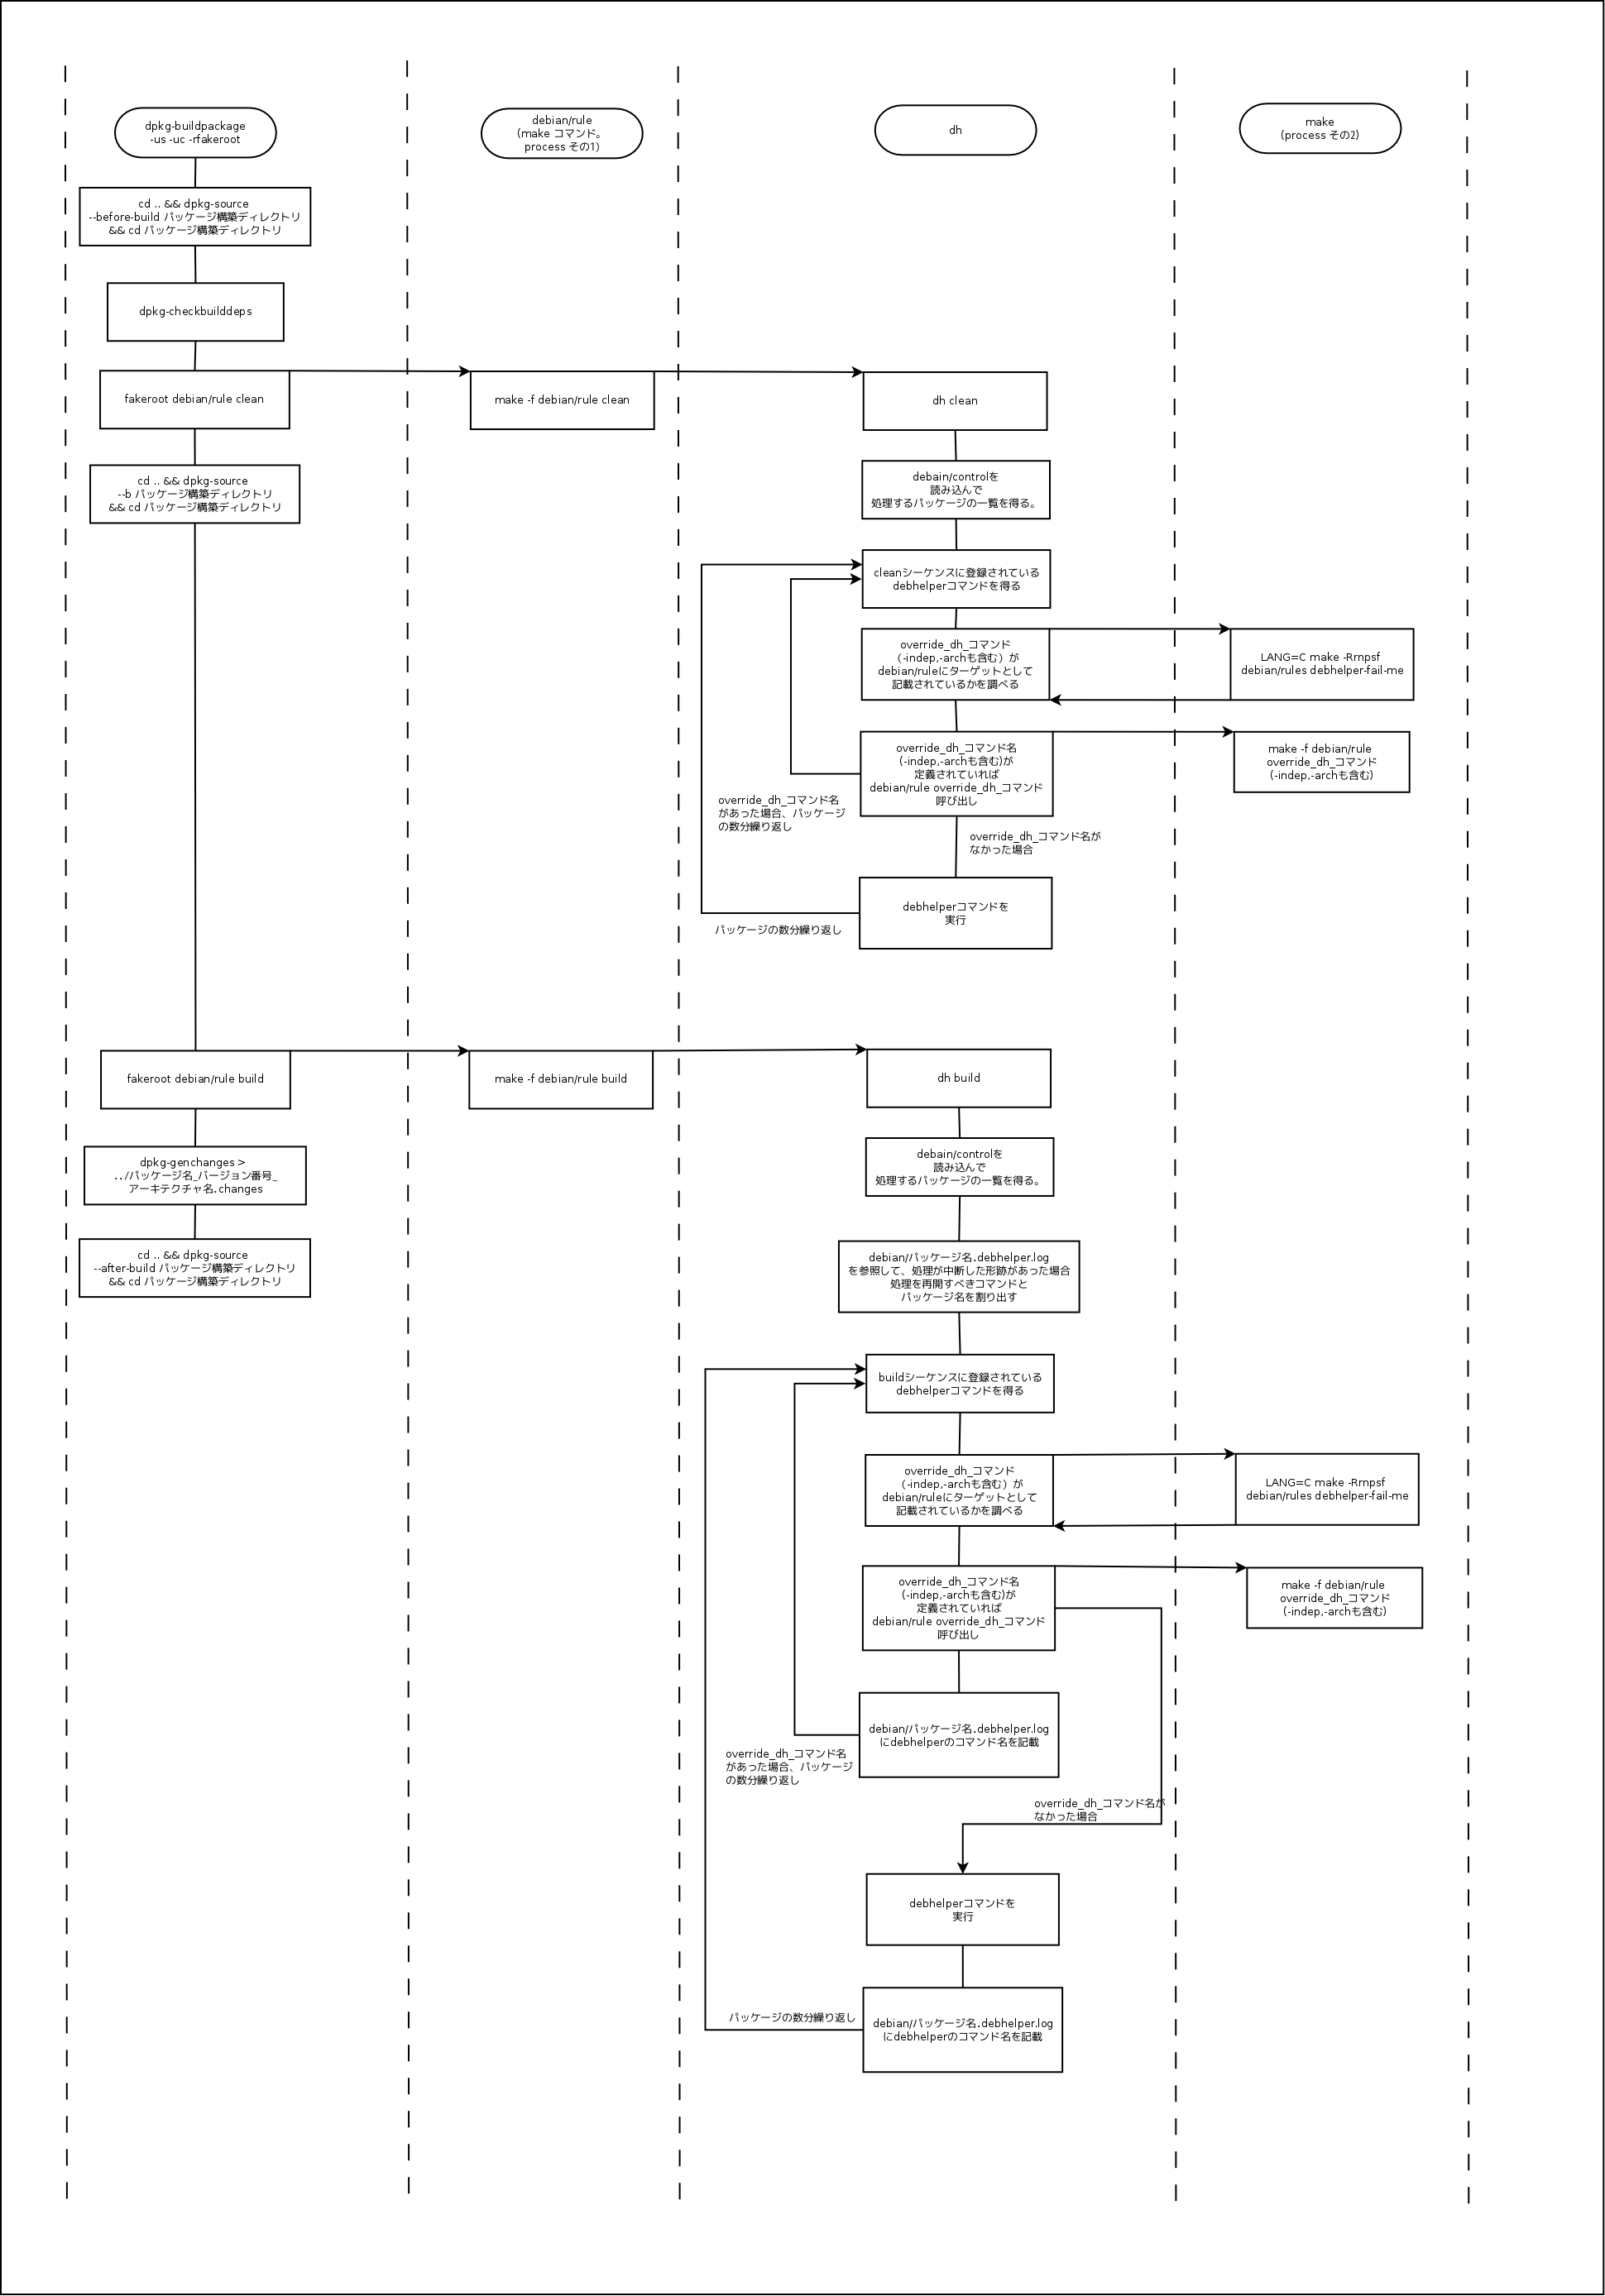
\includegraphics[width=17cm]{image201112/dh-internal-schema1.png}
  \end{center}
  \caption{dh内部動作}
  \label{fig:dh-internal-schema1}
\end{figure}

図\ref{fig:dh-internal-schema1}から判るように、dpkg-buildpackageから
makeコマンドが起動され、次にdhが起動され、
さらにdhからmakeが起動されるという関係になっている事が判ります。また、
override\_{\em debhelperコマンド名}ターゲットの処理を行うのに、makeコマンドを使って
処理をしているという事も判ります。

dhを使うと、makeコマンドはoverride\_{\em debhelperコマンド名}ターゲットの処理をする役目だけを
担当します。
そのうち、dhコマンドが進化すると、makeコマンドの力を借りなくてもパッケージ作成ができるようになる
かもしれませんね。

\subsubsection{``debian/パッケージ名.debhelper.log''ファイルについて}

最近のdhコマンドを使うdebian/rulesには、ファイルの依存関係についての記載がありません。この為、パッケージビルド中で処理が中断した場合、どこから再開すれば良いかをdebian/rulesでmakeが判定する事はできません。

実は、dhコマンドはclean以外のシーケンスが指定されると、''debian/パッケージ名.debhelper.log''というファイルに処理を行ったdebhelperコマンドを記録しています。ここで、万一dhの処理が中断した場合、処理をどこから始めれば良いかについてはこのログファイルを参照して処理の再開を行います。

``debian/パッケージ名.debhelper.log''の中身は以下のようになっています。

\begin{commandline}
debian/パッケージ名.debhelper.logの中身:
dh_auto_test
dh_prep
dh_installdirs
...中略...
dh_buiddeb
\end{commandline}

また、このファイルはdh cleanによって消去されます。なお、dh cleanの時には、このログファイルは作成されません。つまり、dh cleanの処理を中断した場合は、dh cleanは呼び出される一連のdebhelperコマンドは最初から実行されてしまいます。

なお、処理再開の場所は、このログファイルのみ参照して決める為、処理を中断した後に、パッケージのソースファイルを変更して再開させるような使い方はできません。例えば、ソースファイル中のあるファイルを変更した為、特定のパッケージのシーケンスについては再会時に全部やり直しが必要だったとしても、これを自動で検知することはできません。

\subsubsection{dpkg-buildflagとの関係}

dhは互換性度合い(COMPATABLITY LEVEL)のv9から、
パッケージ構築の時に使う環境変数を設定するため、内部でdpkg-buildflag相当の処理を
呼び出します。

その為、9をdebian/compatに指定すると、debhelperコマンドに設定される環境変数は、
\begin{enumerate}
\item /etc/dpkg/buildflags.confの中身
\item XDG\_CONFIG\_HOME/dpkg/buildflags.conf (XDG\_CONFIG\_HOMEは環境変数です)の中身
\item HOME/.config/dpkg/buildflags.conf (HOMEは環境変数です)の中身
\item DEB\_flag\_MAINT\_SET, DEB\_flag\_MAINT\_STRIP, DEB\_flag\_MAINT\_APPEND, DEB\_flag\_MAINT\_PREPEND, DEB\_BUILD\_MAINT\_OPTINS(全部環境変数です)の値
\end{enumerate}
により様々に変化します。どのように変わるかはman dpkg-buildflagを参照してください。

\subsection{今月のコマンドその2:dh\_testroot}

\subsubsection{dh\_testroot動作詳細}

 現在の実行ユーザがrootであるかどうかを確認するコマンドです。rootユーザでは無い場合、
エラーメッセージを出力して処理を中断します。

\subsubsection{dh\_testrootコマンドラインオプション}

 コマンドラインオプションは特にありません。何か指定しても無視されます。

\subsubsection{dh\_testrootを実行してみる}

早速、実行してみましょう。

\begin{commandline}
$ sudo dh_testroot
$ echo $?
0
$ dh_testroot
You must run this as root (or use fakeroot).
$ echo $?
255
$ fakeroot dh_testroot
$ echo $?
0
\end{commandline}
% $

このようにroot権限で実行するか、fakeroot経由で実行した時のみ0を返却します。

\subsubsection{次回の発表について}

次の発表者は勉強会で発表します。選ばれた人はよろしくおねがいします。

%-------------------------------------------------------------------------------
\dancersection{東京エリアDebian勉強会の開催方法}{野島 貴英}
%-------------------------------------------------------------------------------
\index{とうきょうえりあでびあんべんきょうかいのかいさいほうほう@東京エリアDebian勉強会の開催方法}

\subsection{はじめに}

東京エリアDebian勉強会では、毎年12月号資料では勉強会の開催方法についてま
とめています。今回は野島が一通りの流れをまとめます。これを読めば、あなたも
東京エリアDebian勉強会を開けるはず!

\subsection{東京エリアDebian勉強会を開く時のスケジュール}

% 東京エリアDebian勉強会は表\ref{tab:meeting-schedule}のスケジュールで行います。

\begin{table}[ht]
\begin{center}
\small
\begin{tabular}{|p{12em}|p{31em}|}
\hline
時期&作業内容 \\
\hline\hline
開催2ヶ月前 & 場所を確保します。会議室は2ヶ月前に予約しないと埋まりやすいです。\\
\hline
開催2ヶ月前から1ヶ月前 & 勉強会のテーマと、事前課題を決めます。\\
\hline
開催1ヶ月前 & 勉強会のテーマに沿った原稿を募集します。時間枠にあわせた発表が埋まらない場合、発表者を枠が埋まるまで、探す事になります。また、開催にあたり、作業の分担が必要な時は、この時ぐらいに割り当てを完了します。また、宴会の場所について、確保が困難な事が予想される場合は、あらかじめ席のみ予約しておきます。\\
\hline
開催2週間前までに & Debian勉強会予約システム\url{http://debianmeeting.appspot.com}に予約登録ページを作成します。Debian JP Blog \url{http://www.debian.or.jp/}及び、Debian勉強会Webサイト \url{http://tokyodebian.alioth.debian.org/} に勉強会の内容を提示します。
     メールで debian-users メーリングリストにアナウンスを投げます。
     debian JP twitter や mixi Debian コミュニティーなどにもアナウンスす
     ることが多いです。\\
\hline
開催1週間前 & 発表者は勉強会資料用リポジトリに資料をコミットします。\\
\hline
開催2日前 & 参加者の募集の締切りを行います。この時までに揃った事前課題を勉強会資料にマージします。\\
\hline
開催1日前 & kinkos等の印刷製本サービスに原稿印刷および製本を依頼します。\\
\hline
開催当日 & \begin{enumerate}
  \item 参加者から費用の回収と集計をします。
  \item 勉強会を定刻どおりに開催します。
  \item 司会者、発表者と協力して時間内に勉強会を終了します。
  \item 宴会の場所の確保が困難でない時は、宴会の場所を抑えます。
  \item 宴会の開催、宴会の会計をします。
\end{enumerate} \\
\hline
開催後 & Debian勉強会予約システムからアンケートをおくります。 \\
\hline
12月 & 勉強会のアンケート結果などを一年分集計して発表します。 \\
\hline
\end{tabular}
\caption{全体スケジュール}
\label{tab:meeting-schedule}
\end{center}
\end{table}

\subsection{東京エリアDebian勉強会の開催調整}

東京エリアDebian勉強会の開催調整は専用のMLがあり、普段はこちらで調整が行われます。
運営者専用のMLで、一部のコアメンバーのみが参加しています。
運営に積極的に参加したい人は勉強会運営者に連絡を取る必要があります。

\subsection{初めて東京エリアDebian勉強会の開催を担当する場合の事前準備}

初めて東京エリアDebian勉強会の開催を担当する場合以下の項目が準備してあると
スムーズです。

\begin{enumerate}
\item Debian JP Projectの提供するサーバーへログインできるアカウント\\
Debian JP Blogを更新する際に必要になります。
これは通常Debian JP Projectの会員になるときに付与されます。
会員でない人は会員にコミットしてもらうよう依頼する必要があります。

\item \url{http://alioth.debian.org/}アカウント
資料の編集等を行う際に必要になります。
アカウントを取得したら、MLでtokyodebianグループ権限に所属させてほしい旨、
取得したアカウント名を沿えて依頼します。このアカウントは誰でも取得可能です。

% ここはgmailアカウントがあれば誰でもできる。ので削除。
%\item \url{http://debianmeeting.appspot.com/}を操作できるように、
%MLで依頼します。この時、開催しようとしている勉強会のイベント登録ページも作成してもらいます。

\end{enumerate}

また、勉強会の幹事担当の場合に必要な知識とコンピュータの環境は以下になります。

\begin{enumerate}
\item Debianが動作し、インターネットが利用できるPCの用意
\item ssh,emacs,muse-el,git、subversionの基本操作についての知識
\item ブラウザとHTMLの記載の知識
\item \url{http://alioth.debian.org/},\url{http://qwik.jp/}の使い方の知識
\item \LaTeX{}の知識
\end{enumerate}

わからないことや困ったことがあればメールやMLで聞いてみましょう。

\subsection{東京エリアDebian勉強会の掲示の出し方}

\url{http://www.debian.or.jp/}に掲示を出す場合の編集の仕方は、
\url{http://www.debian.or.jp/project/webmasters.html}にその記載があります。
実際には、svnでリポジトリをとってきて、
www.debian.or.jp/blosxom/ data/events/tokyodebian-XX.d (XXは第XX回を示します)を
作成します。

\url{http://debianmeeting.appspot.com/eventadmin/edit?eventid=}のフォームの編集
はフォームに沿って情報を入れるだけです。ただ、細かい事は、\url{http://tokyodebian.alioth.debian.org/YYYY-MM.html}へのリンクをURLの
欄に指定し、細かい事はそちらを参照してもらいます。

\url{http://tokyodebian.alioth.debian.org/}へは、\url{http://qwik.jp/ML名}のトップ
ページに記載されているやり方に従います。実際にはgit
で\url{git+ssh://git.debian.org/git/tokyodebian/muse.git};リポジトリをcloneして、muse形式で編集し、make publishする事となります。

\printindex

\cleartooddpage

\vspace*{15cm}
\hrule
\vspace{2mm}

\includegraphics[width=2cm]{image200502/openlogo-nd.eps}
\noindent \Large \bf Debian 勉強会資料\\
\noindent \normalfont \debmtgyear{}年\debmtgmonth{}月\debmtgdate{}日 \hspace{5mm}  初版第1刷発行\\
\noindent \normalfont 東京エリア Debian 勉強会 (編集・印刷・発行)\\
\hrule

\end{document}
